\documentclass[letterpaper, 12pt]{report}
\usepackage{style} % requires style.sty
\pgfplotsset{compat=1.18} % Use a modern compatibility version

% --- This block defines the styles for each line ---
\pgfplotsset{
    % Style for the 'Constant' line
    style-constant/.style={
        blue,
        solid,
        mark=*,
        mark size=4pt, % Much larger markers
    },
    % Style for the 'Adversarial' line
    style-adversarial/.style={
        red,
        solid,
        mark=square*,
        mark size=4pt, % Much larger markers
    },
    % Style for the 'Benevolent' line
    style-benevolent/.style={
        black, % The line color
        solid,
        mark=otimes*, % Circle with a cross (X)
        mark size=4pt, % Much larger markers
        mark options={ % --- This sets the mark colors ---
            draw=black, % The black outline and black X
            fill=brown   % The brown fill color
        }
    },
    % Style for the 'Oblivious' line
    style-oblivious/.style={
        green!60!black, % A darker green
        solid,
        mark=star,
        mark size=3pt, % Much larger markers
    }
}

\begin{document}

% Using a 'figure' environment is good practice
\begin{figure}[ht!] 
\centering % Center the figure
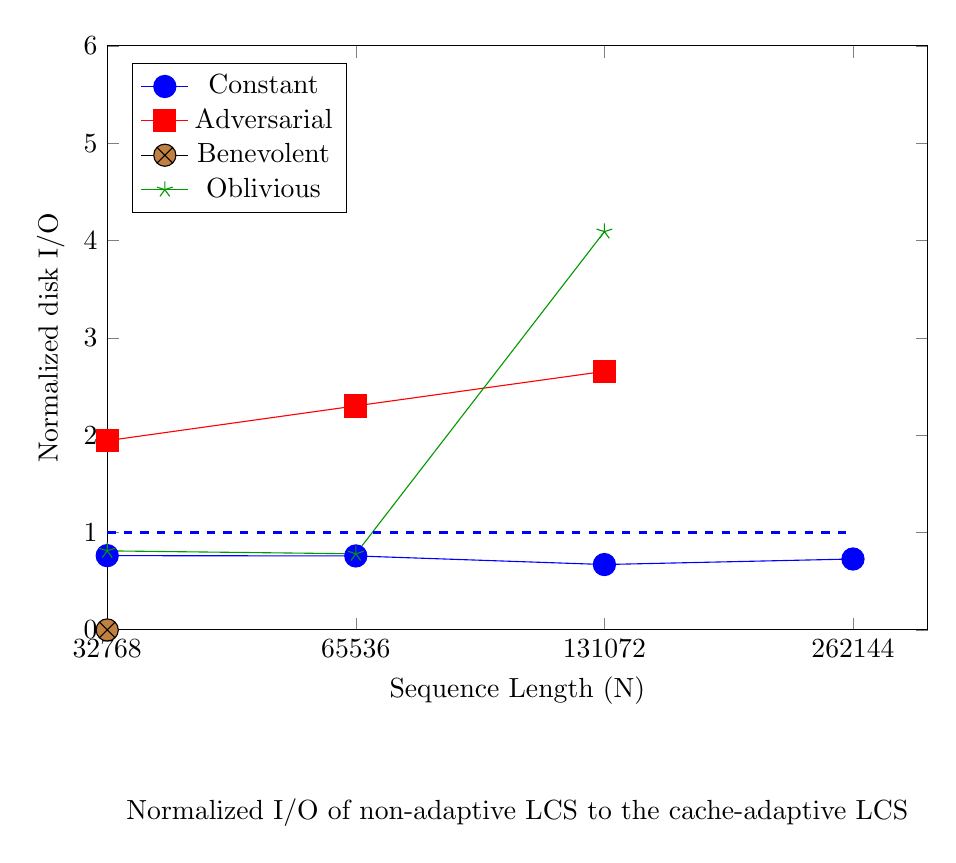
\begin{tikzpicture}
\begin{axis}[
        % --- Main Axis Settings ---
        width=12cm, % Adjust size as needed
        height=9cm,
        xmode=log,    % X-axis is logarithmic
        xlabel={Sequence Length (N)},
        ylabel={Normalized disk I/O},
        % --- Y-Axis Settings ---
        ymin=0, ymax=6,
        ytick={0, 1, 2, 3, 4, 5, 6},
        % --- X-Axis Settings ---
        % Use the exact ticks from your graph
        xmin=32768, % Start x-axis at 32768 to eliminate left gap
        xtick={32768, 65536, 131072, 262144},
        xticklabels={32768, 65536, 131072, 262144}, % Ensures labels match ticks
        % --- Legend Settings ---
        legend pos=north west,
        % --- Title/Caption Setting ---
        % This places the '(b) ...' text below the x-axis label
        title={Normalized I/O of non-adaptive LCS to the cache-adaptive LCS},
        title style={at={(0.5, -0.3)}, anchor=north}
    ]
    
    % --- PLOT 1: Constant ---
    \addplot[style-constant] coordinates {
        (32768, 0.763324)
        (65536, 0.760135)
        (131072, 0.671801)
        (262144, 0.728745)
    };
    \addlegendentry{Constant}
    
    % --- PLOT 2: Adversarial ---
    \addplot[style-adversarial] coordinates {
        (32768, 1.943950)
        (65536, 2.301401)
        (131072, 2.655752)
    };
    \addlegendentry{Adversarial}
    
    % --- PLOT 3: Benevolent ---
    \addplot[style-benevolent] coordinates {
        (32768, 0)
    };
    \addlegendentry{Benevolent}
    
    % --- PLOT 4: Oblivious ---
    \addplot[style-oblivious] coordinates {
        (32768, 0.812267)
        (65536, 0.782044)
        (131072, 4.091529)
    };
    \addlegendentry{Oblivious}
    
    % --- REFERENCE LINE: y=1 ---
    \addplot[blue, dashed, thick] coordinates {
        (32768, 1)
        (262144, 1)
    };
    
    \end{axis}
\end{tikzpicture}
\end{figure}

\end{document}
